\subsection{ISO-Normenreihe 9241 zur Gebrauchstauglichkeit und Ergonomie interaktiver Systeme}
\label{ch:SdF:UI:ISO}

Die Normen unter der DIN EN ISO 9241 aus dem Jahr 2020 geben Vorgaben und Empfehlungen zur Gestaltung interaktiver Systeme.
\autoref{fig:iso-uebersicht} stellt den Zusammenhang der Hauptquellen für Empfehlungen zur Benutzer-System-Interaktion dar. Es sind die Parts 11, 110, 112 und weitere zu erkennen. Die DIN EN ISO 9241-11 definiert den Begriff Usability, %(dt. Gebrauchstauglichkeit)
währenddessen Part 110 und 112 Prinzipien und Grundsätze mitgeben, um die Usability eines Systems gewährleisten zu können.

\begin{figure}[H]
    \centering
    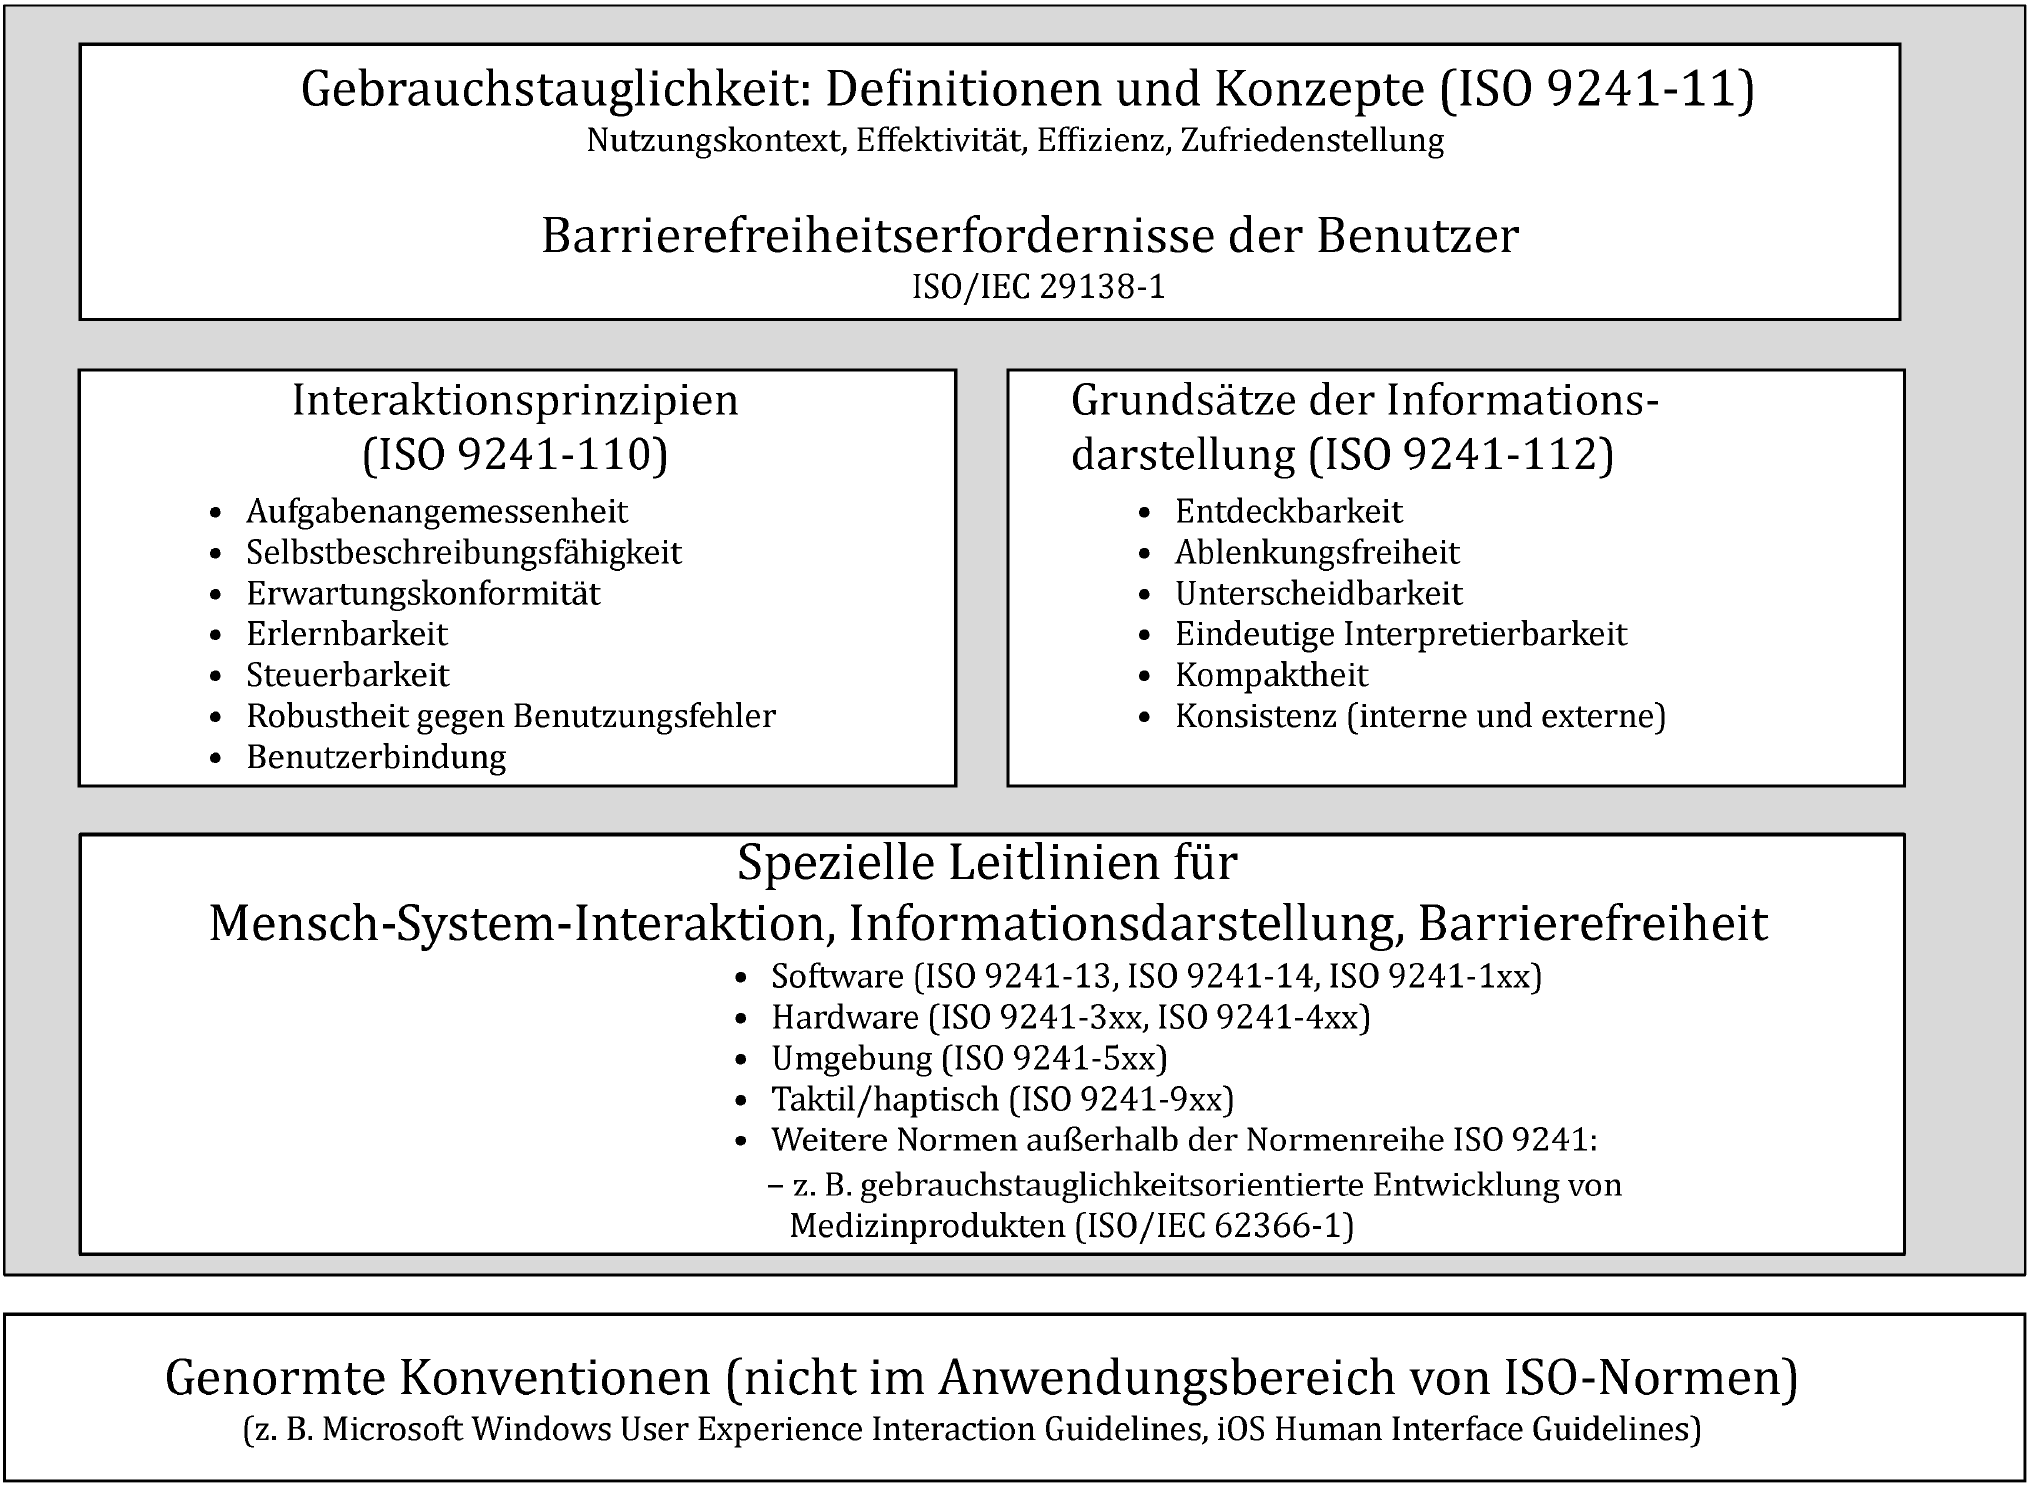
\includegraphics[width=1\linewidth]{chapters/02_Stand_der_Forschung/ISO-Normen_Uebersicht.PNG}
    %\caption{Überblick und Zusammenspiel der ISO-Normen mit Fokus auf die Usability von interaktiven Systemen \cite{DIN_EN_ISO_9241-110}}
    \caption{\glqq Beziehung zwischen den Hauptquellen für Empfehlungen zur Benutzer-System-Interaktion\grqq{} \cite{DIN_EN_ISO_9241-110} mit Fokus auf die Usability}   % S. 16
    \label{fig:iso-uebersicht}
\end{figure}

\noindent
%In den folgenden Kapiteln werden die Inhalte der DIN EN ISO 9241-110 Interaktionsprinzipien (ISO 9241-110:2020) \cite{DIN_EN_ISO_9241-110} mit Fokus zur Anwendung auf Dashboards zusammengefasst.
Die DIN-Normen sind in diesem Fall die nationale Umsetzung der internationalen ISO-Normen und werden nachfolgend synonym mit ‚ISO‘ referenziert.
